\documentclass{jsarticle}

\usepackage[dvipdfmx]{graphicx}

\title{アカタテハ観察日誌}

\begin{document}
\maketitle

\section{5/30の記録}
\subsection{14時:舞岡公園}
この日は, ブログなどの記事から, 横浜市の舞岡公園というところが, ゼフィルスがよく発生しており, 
去年, 今年に更新されたような新しいブログもあることから, 今年でも観察で来ると思い, 
さらに, ブログでのゼフィルス観察記録時期がちょうど今頃なので, 行って見ることにした. 

実際に公園について見ると, 四季の森公園と比較して, いわゆる公園, という印象が強く, 蝶の姿もほとんど見られなかったが, 
公園の中を歩いていると, 目当ての一つである, ウラゴマダラシジミと思われる, 飛翔体が1体見つかった. 
ルリシジミが大きく, 早くなったような飛び方をする印象がある. 

さらに奥に進んでいくと, 門を界に, 一気に雰囲気が変わり, いかにも自然公園という雰囲気になってきた. 
植物も, 自然のままのものが生い茂り, また, コナラの木が非常に多く, ゼフィルスが多いのも納得できる. 

さらに奥に進んでいくと, 田植えをしているエリアがあり, ここで急に蝶の数が増え始めた. 
ベニシジミや, おそらくスジグロシロチョウ, モンシロチョウ, モンキアゲハ, キタテハ, ゴマダラチョウ, アオスジアゲハなどが見られた. 
また, 田んぼのそばに, まだ見分ける自身がないが, おそらくイボタと思われる木が何本か生えており, この周りに, ウラゴマダラシジミが飛んでいた. 

その先に進んでいく林道では, 何度もウラゴマダラシジミが見つかり, 数が多いのだと実感した. 
ただ, ウラゴマダラシジミは, 一度も止まることがなかったので, 撮影することができなかった. 一体どうやって撮影するのだろうか. 

\subsection{15時:イラクサ系の植物に, 巣を発見}
進みながら, ヤマノイモの食痕のある葉をひっくり返すも, ダイミョウセセリの幼虫はまったく見つからず. 
カタバミの食痕をひっくり返すもヤマトシジミの幼虫も見つからず. サルトリイバラの葉をひっくり返すもルリタテハの幼虫は見つからず. まあ, ルリタテハ以外は, そもそも幼虫を見たことがないのだからとんちんかんな探し方をしている可能性も大だが. 
そんななか, ふと見たイラクサ系の植物に, 見慣れた巣があるのを発見, のぞいて見ると, 明らかに中でトゲトゲの何かが動いている. 
これはアカタテハに違いないと確信. 持って帰ることとした. 

\subsection{18時:巣を破壊, 新しい葉に移動}
巣は完全に枯れていたので, 申し訳ないが破壊して開いてみると, 間違いなくアカタテハの幼虫であった. サイズからしておそらく3齢程度か. 

\begin{figure}[htbp]
  \begin{center}
    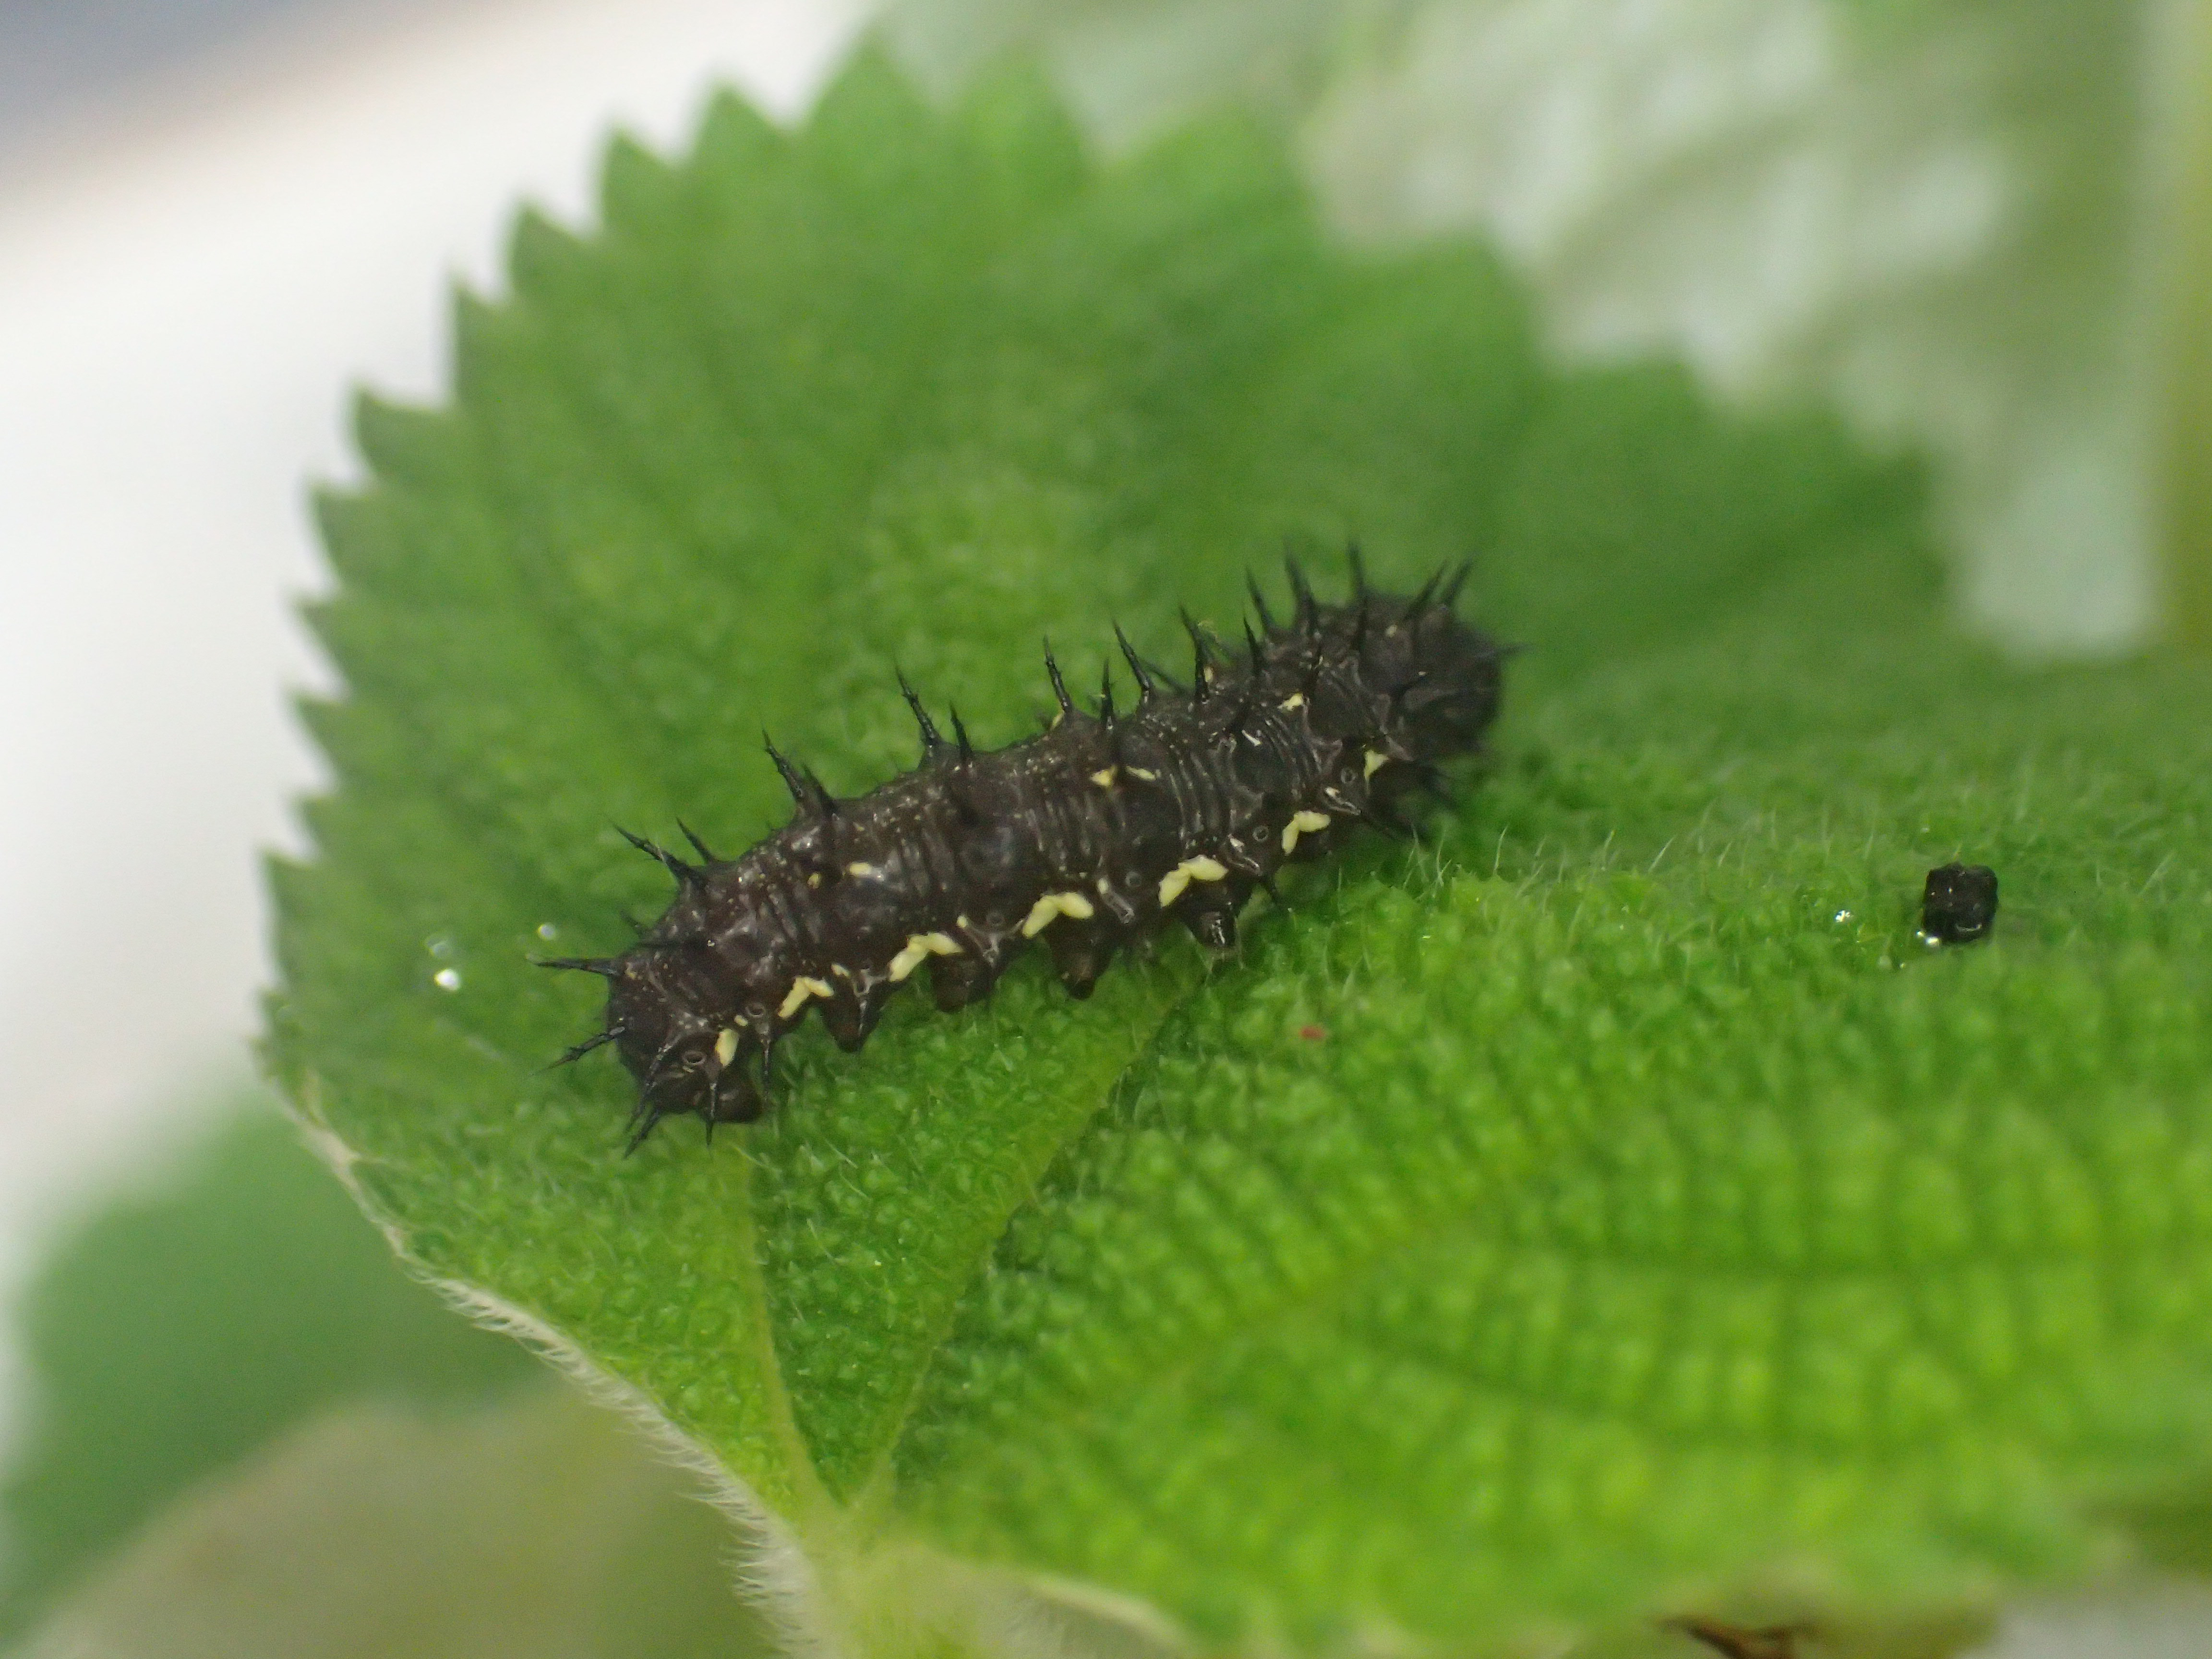
\includegraphics[width=5cm]{photo1/Larva.JPG}
  \end{center}
  \caption{アカタテハの幼虫}
\end{figure}

すぐに食草を取りに行った. 鶴見川沿いに沢山自生していたのを思い出し, 採取してきた. 
あまり知らなかったが, アカタテハの食草になるような, イラクサ系の植物には, カラムシ, ヤブマオ, クサマオといった植物があるようだが, 舞岡公園のは確認していないが, 鶴見川沿いのものはカラムシであった. 

\subsection{24時:新しい巣を早速作成していた}
巣から引きずり出された幼虫は, やはりまっさきに巣を作ろうとするようで, 巣ができていた. 
ただ, その後改めて観察すると, 巣から出て, 別の葉の上に堂々といるときもあり, 必ずしも引きこもりなわけではないようだ. 

\begin{figure}[htbp]
  \begin{center}
    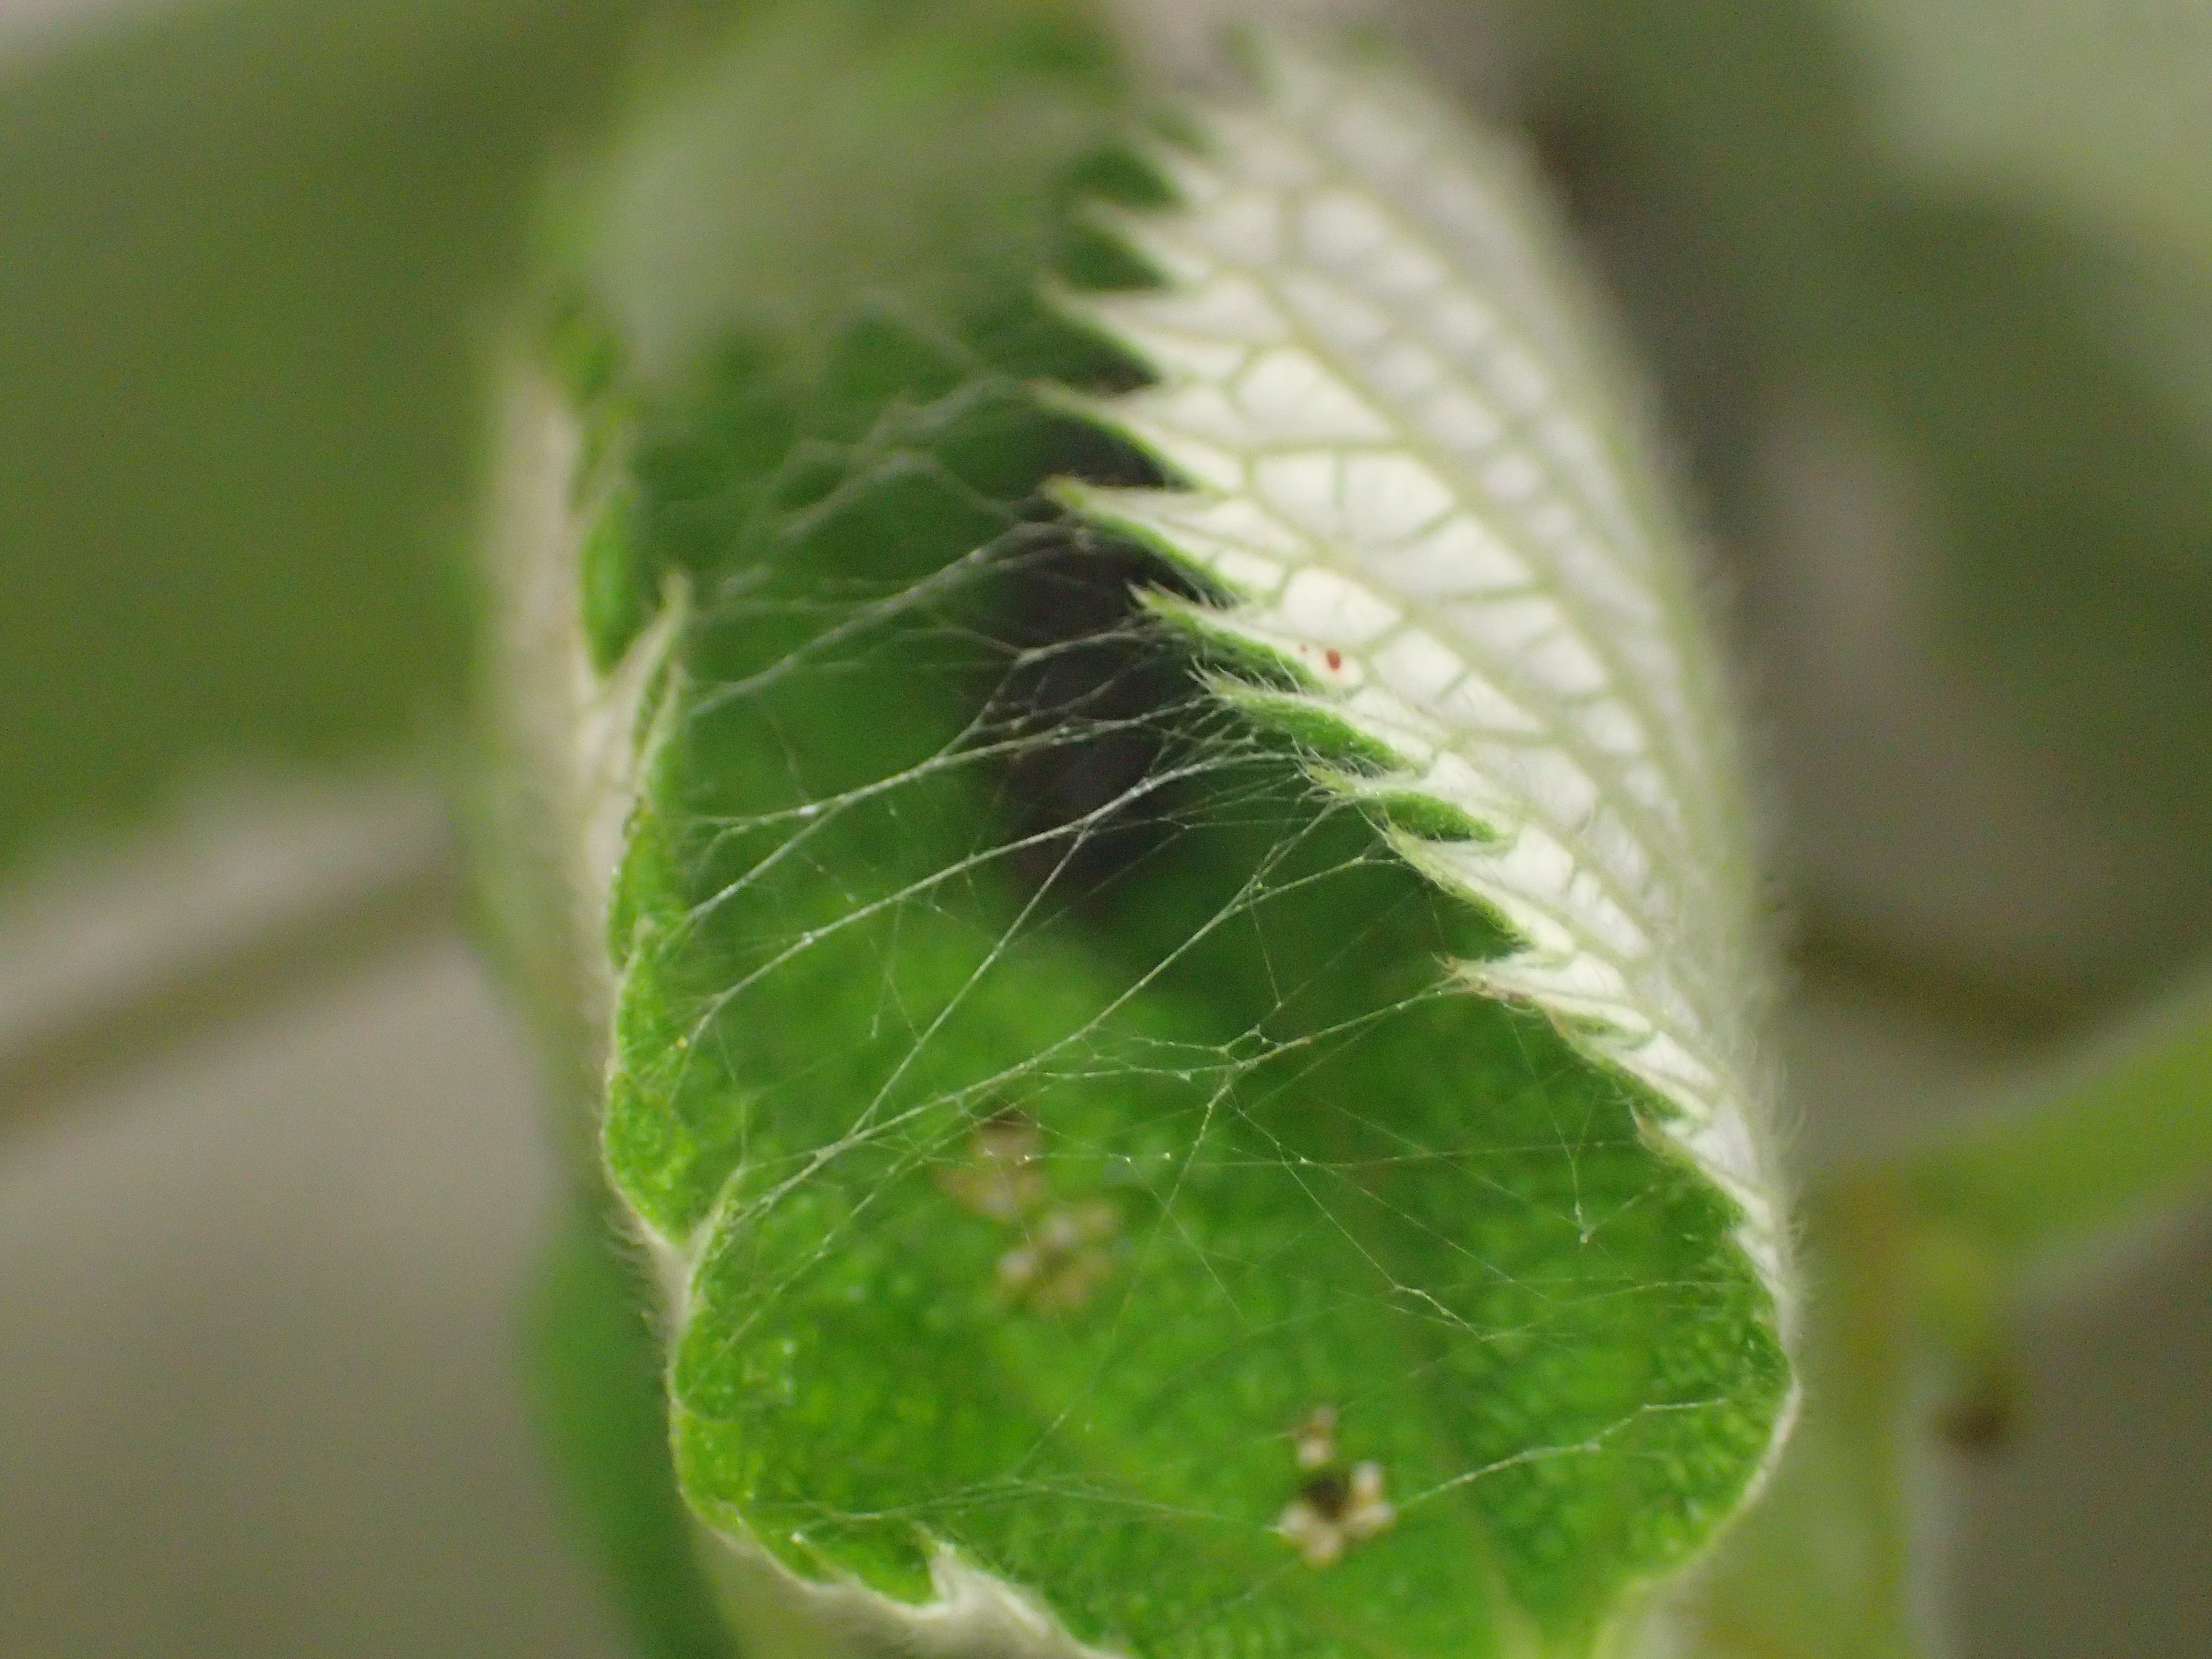
\includegraphics[width=5cm]{photo1/Larva-nest.JPG}
  \end{center}
  \caption{新しい巣ができていた}
\end{figure}

\section{5/31の記録}
\subsection{10時:あまり食べない}
幼虫は, あまり多く食べておらず, 巣の一部が少し透けている程度であった. 食草はヤブマオの方がよかったか. 

\subsection{13時:もう一個巣を作っていた}
何か気に入らなかったのか, それとも身を守るためのダミーなのか, 二個目の巣を作っていた. 

\begin{figure}[htbp]
  \begin{center}
    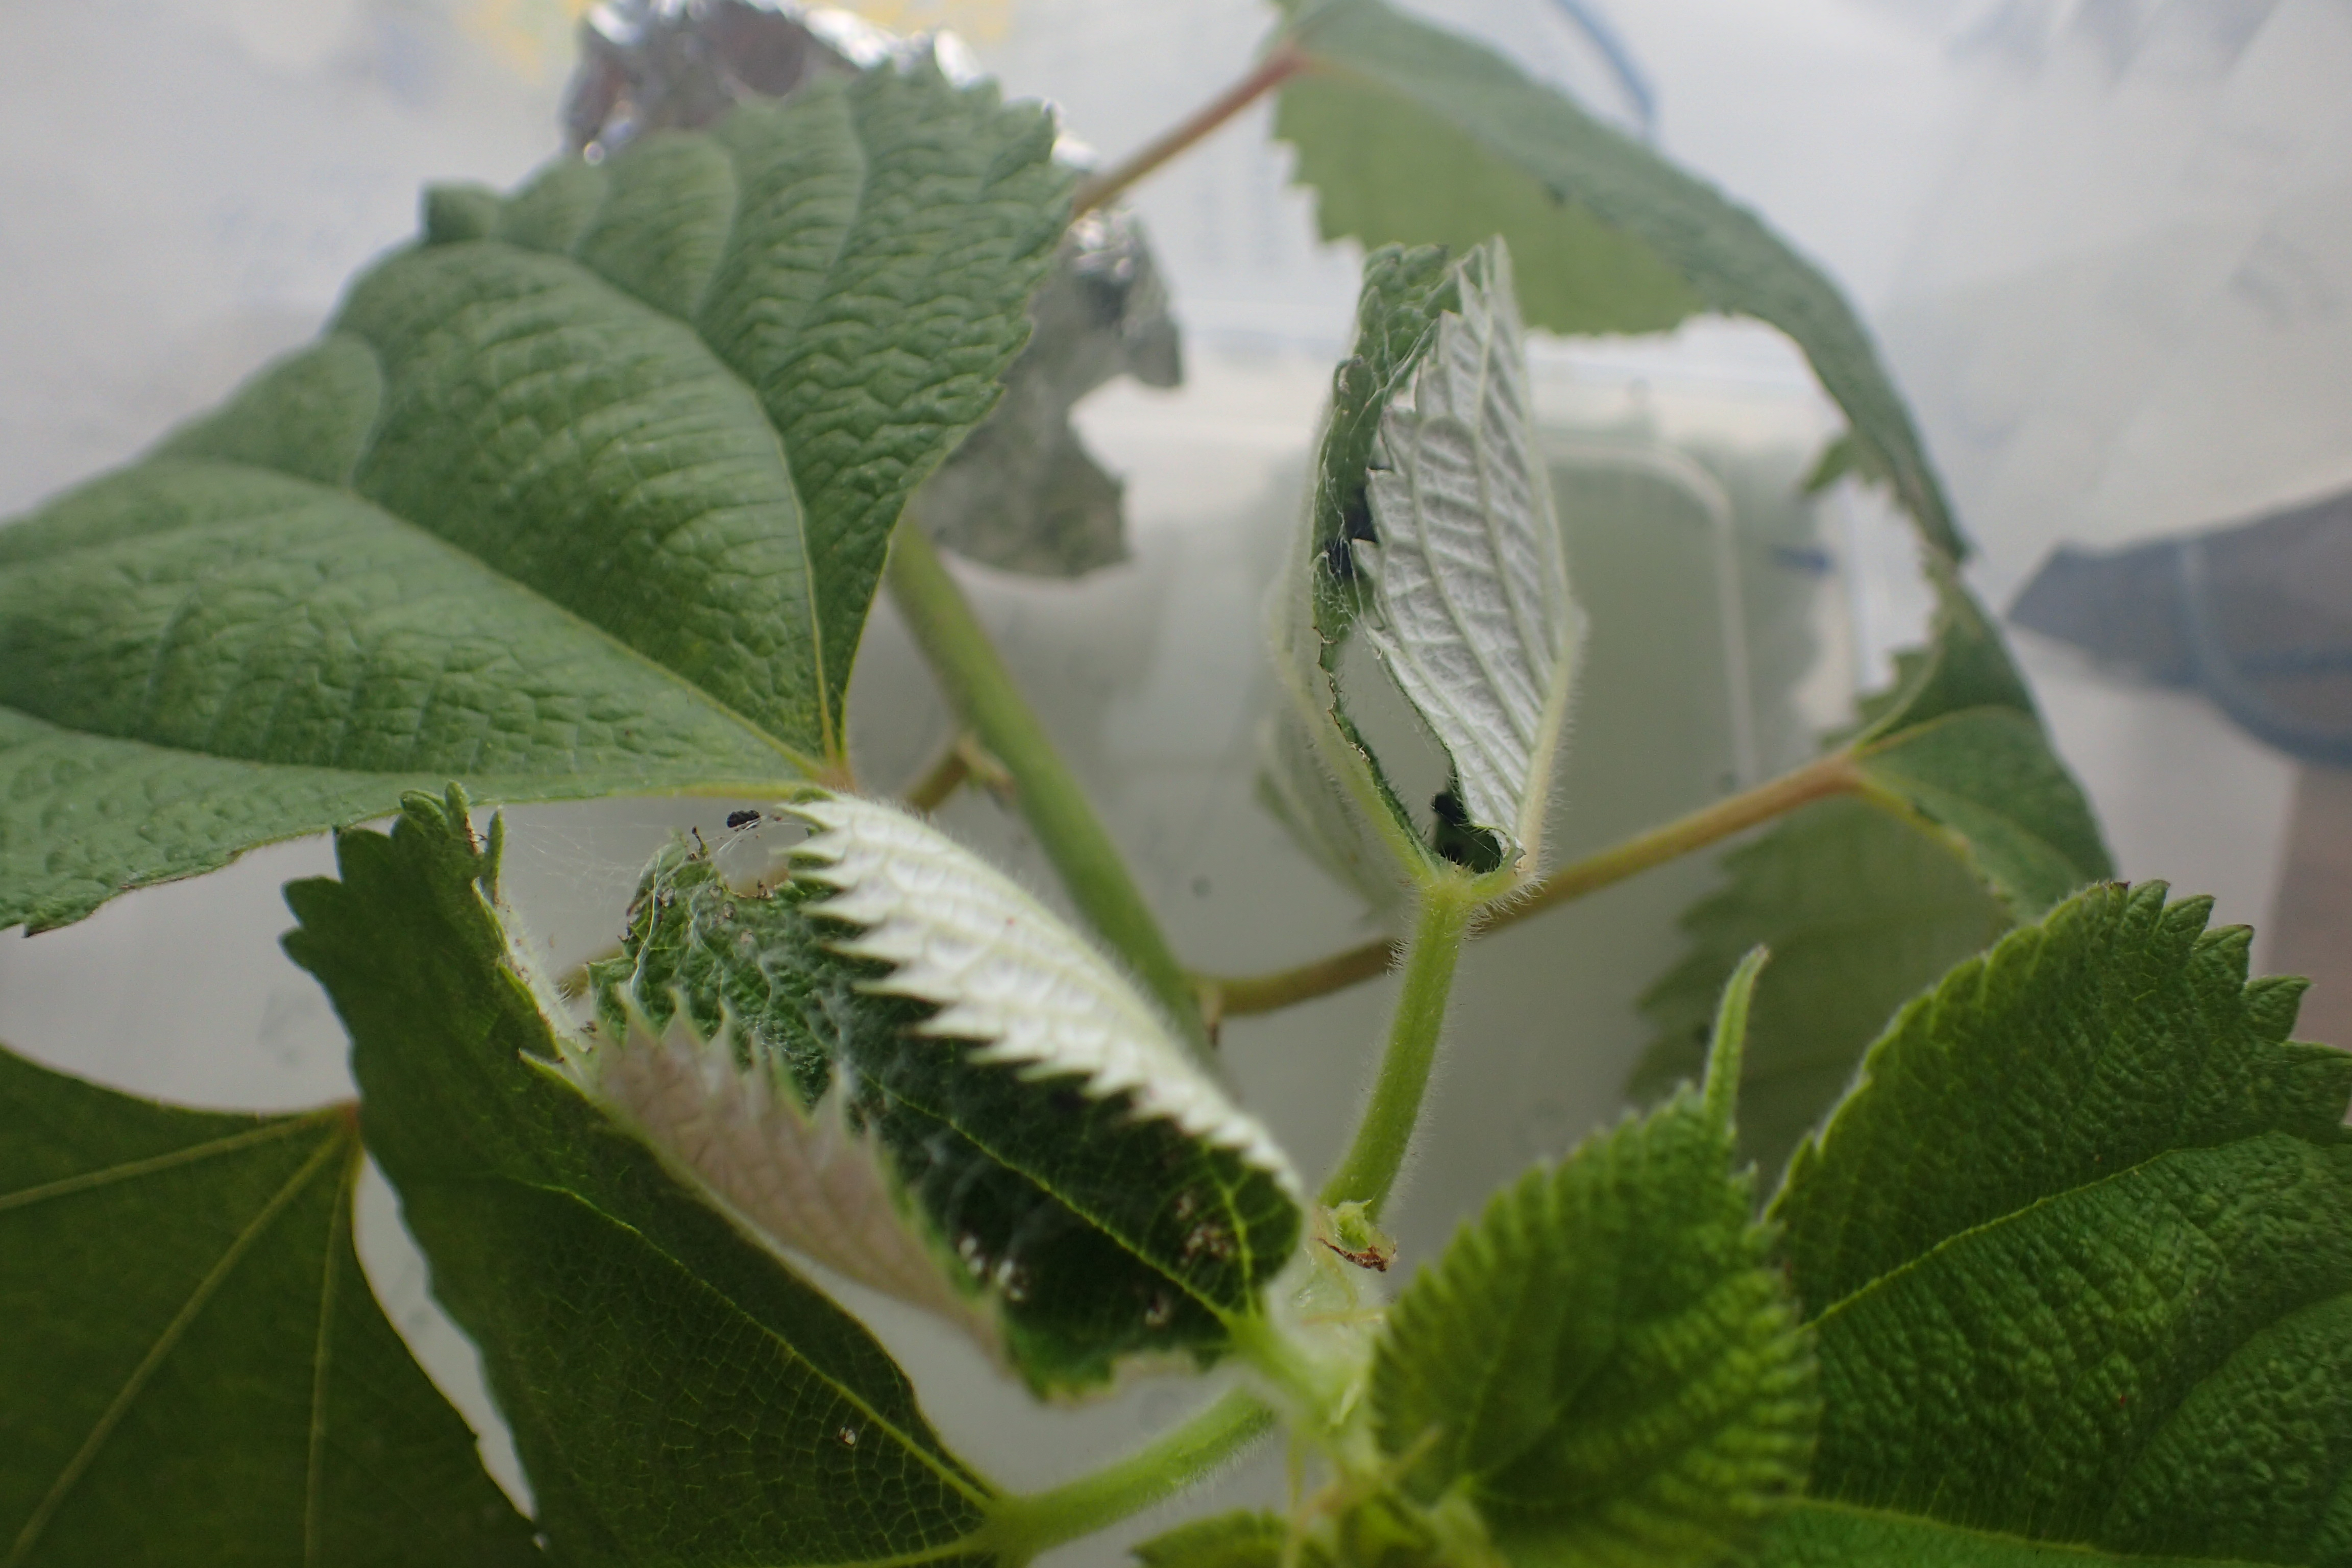
\includegraphics[width=5cm]{photo2/Larva-nest.JPG}
  \end{center}
  \caption{さらに新しい巣ができていた}
\end{figure}

\section{6/1の記録}
\subsection{23時:基本的に巣しか食べないようだ}
幼虫が餌を食べないなと思っていたが, 基本的に巣に穴を開けるような食べ方しかしないようだ. 
アカタテハは, 巣にこもりきりなので, 観察があまり面白くない. 

\begin{figure}[htbp]
  \begin{center}
    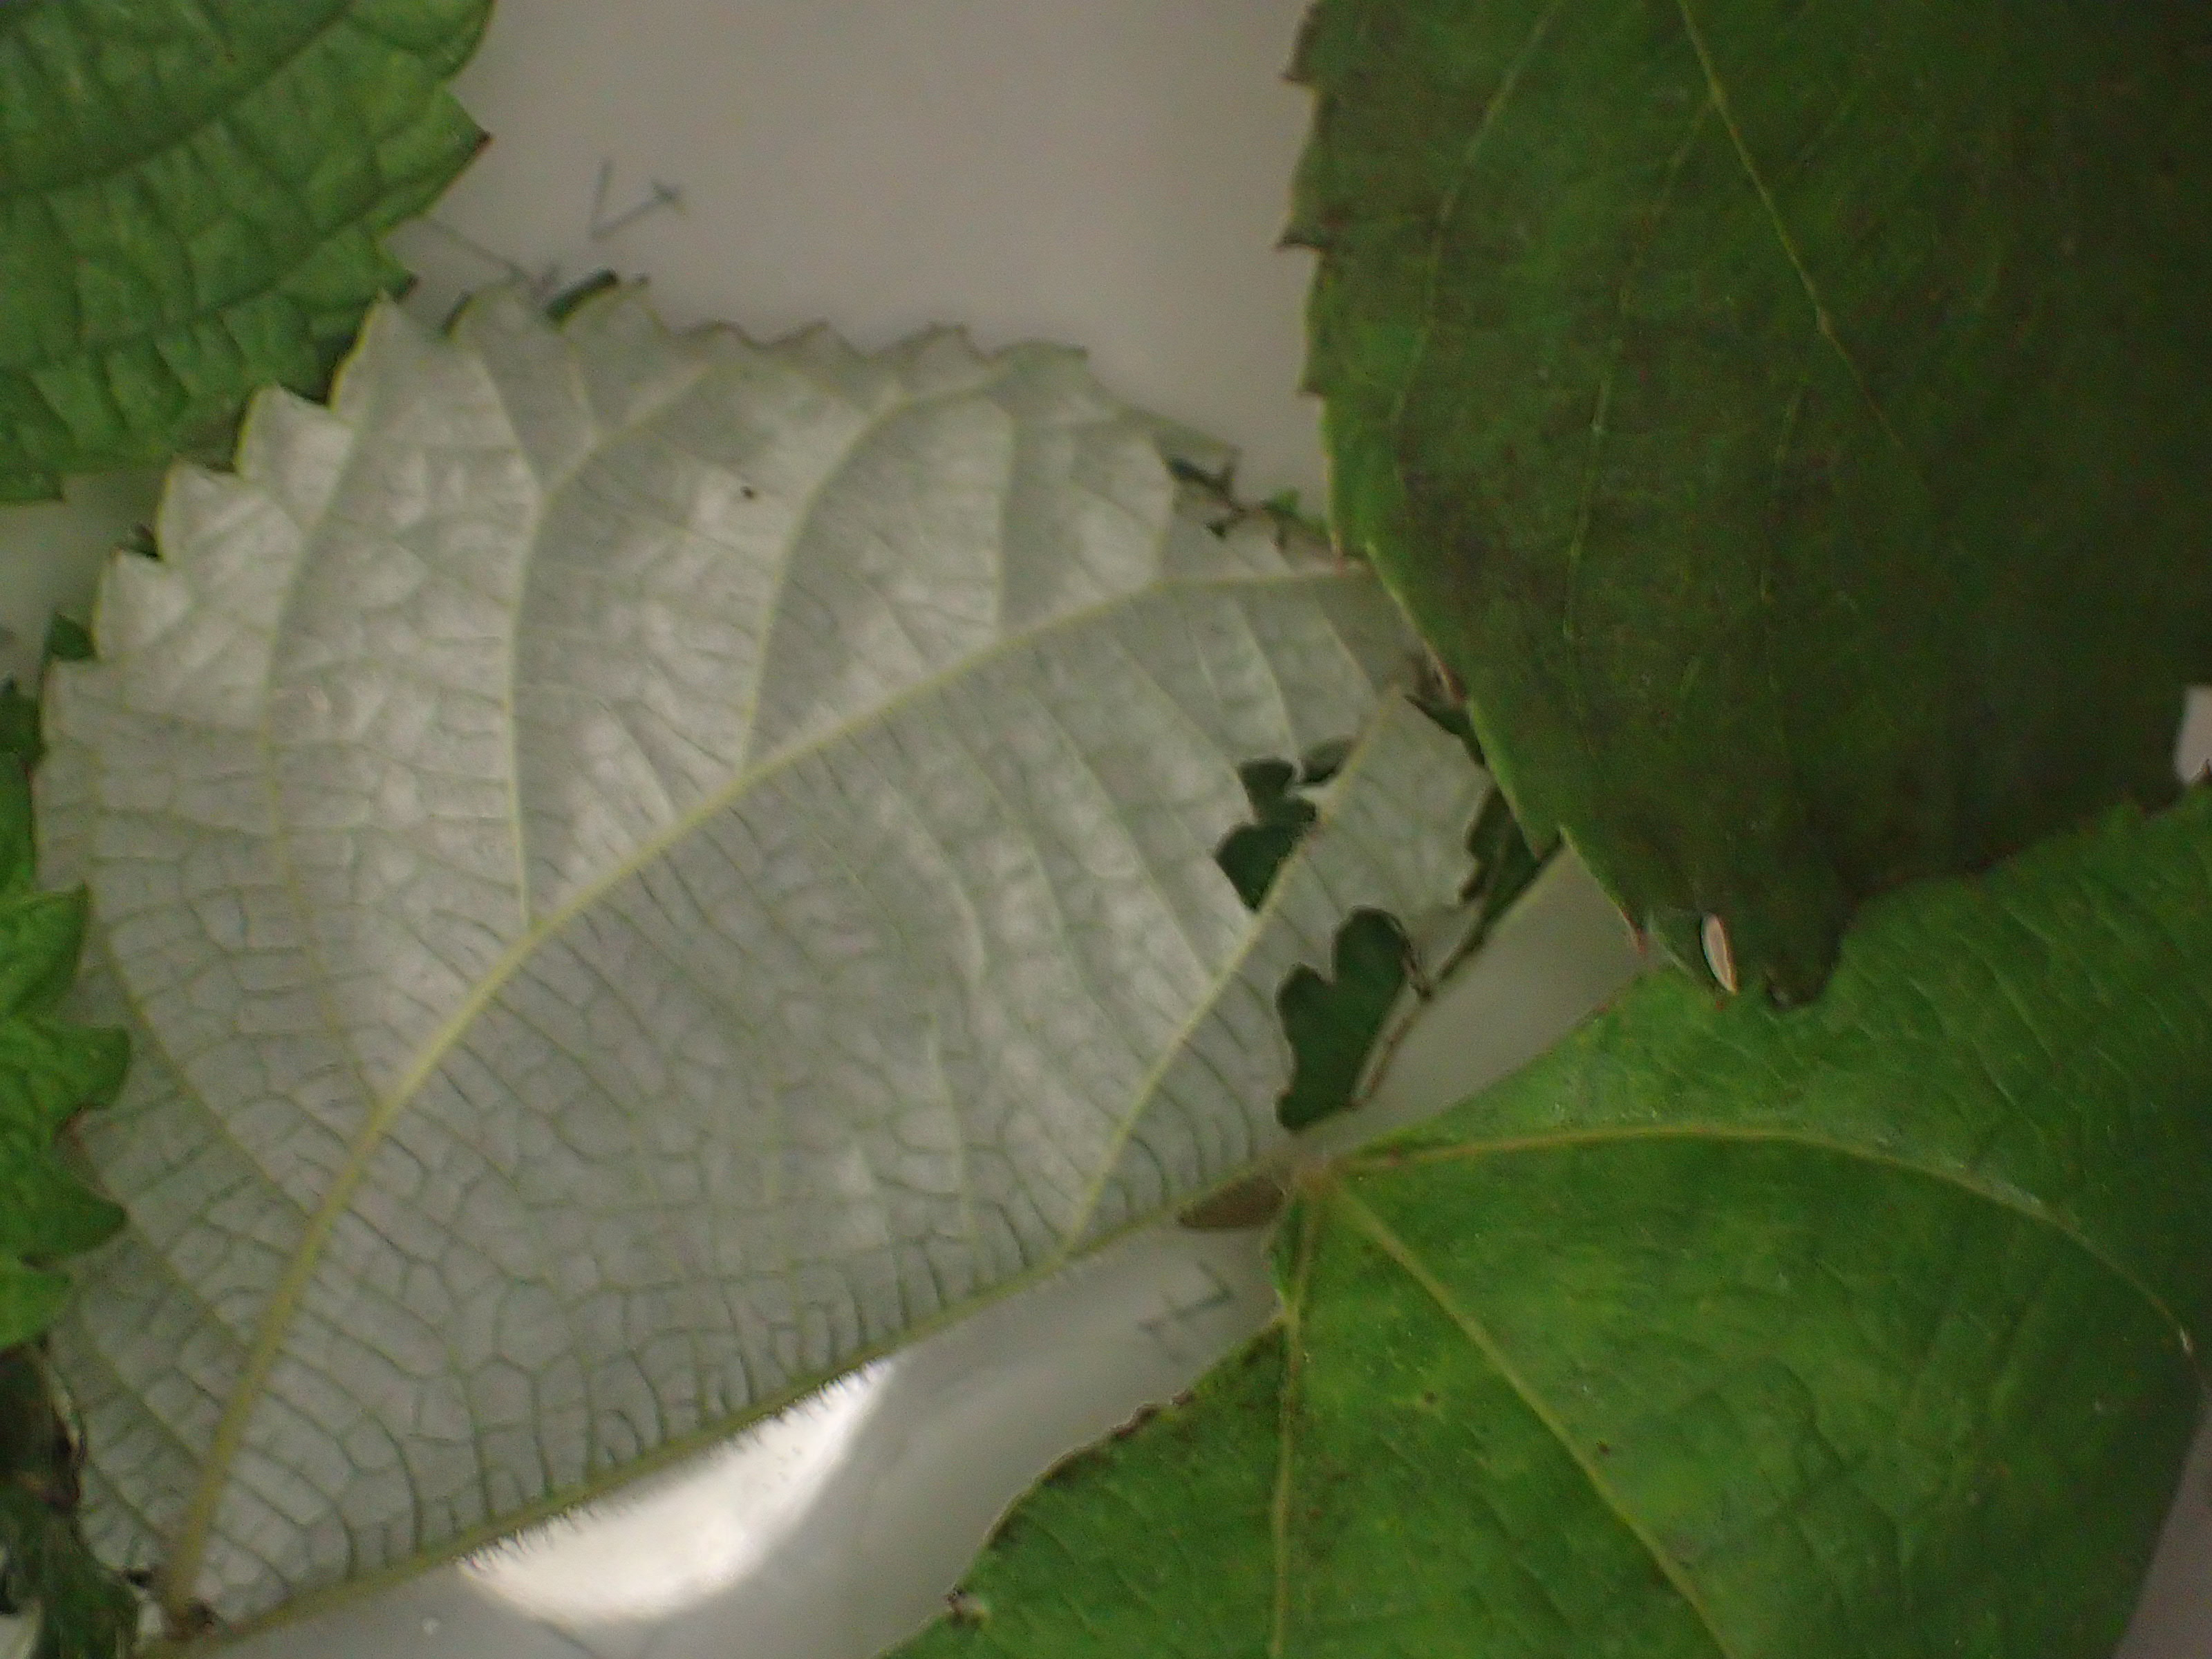
\includegraphics[width=5cm]{photo3/bitemark.JPG}
  \end{center}
  \caption{巣に食痕}
\end{figure}

\section{6/3の記録}
だいぶ食草がしおれてきており, 交換しようと思っていたところ, 幼虫が巣から這い出して動いていた. 
さすがに, 食草が枯れてきたら引っ越すようだ. 
新しい葉で, 巣を作っていたが うまいこと, 若い葉, 大きい葉をまきこんだ巣にできたようで, 
食べるときはわかい葉を食べていた. いつの間にか少し大きくなっていた. 

\section{6/6の記録}
前蛹になっていた. 

\section{6/7の記録}
蛹化していた.

\end{document}
